\documentclass{report}
\usepackage{amsmath}
\usepackage[pdftex]{color,graphicx}
\usepackage{listings}
\usepackage{ textcomp }

\usepackage{xcolor}
 
\usepackage{float}


\begin{document}
 Parallizaiton of the code.\\
 The whole calculation of this code is a iteration procedure. Matrix Psi is the matrix of streamlines and matrix Omega is the matrix of vortices. Matrix Psi is calculated in function PsiCalc with an iterative method. Fuction PsiCalc is the most time consuming function in the serial version of this code. It may need several or tens of iterations to finish. As a finite element problem,new Psi  and Omega matrices are calculated from the old Psi and Omega matrices. Every elements in new Psi and omega matrix is a function of 5 elements in the old matrix.\\
   $New\_Psi[i][j]=Function( Old\_Psi[i][j],Old\_Psi[i-1][j],Old\_Psi[i+1][j],Old\_Psi[i][j+1],Old\_Psi[i][j-1] )$\\
 For the parallelization scheme, a processor only store and calculate a part of the Psi and Omega matrix. The Psi and omega are all (Nx+2)*(My+2) matrix. They both have two rows at the top and bottom and two columns at the right and left that considered as boundary, which are set in the BCs function. We use a highly symmetric configuration for parallelization. Every processors calculate and store a (nx+2)*(my+2) matrix.They also have  two rows at the top and bottom and two columns at the right and left that are considered as boundary. And they do not calculate the boundary. Small matrices  overlap with the adjacent matrix with two rows or tow columns. The boundary of each processors are calculated by other processors.
 
 
 \begin{figure}[H]
 \begin{center}
 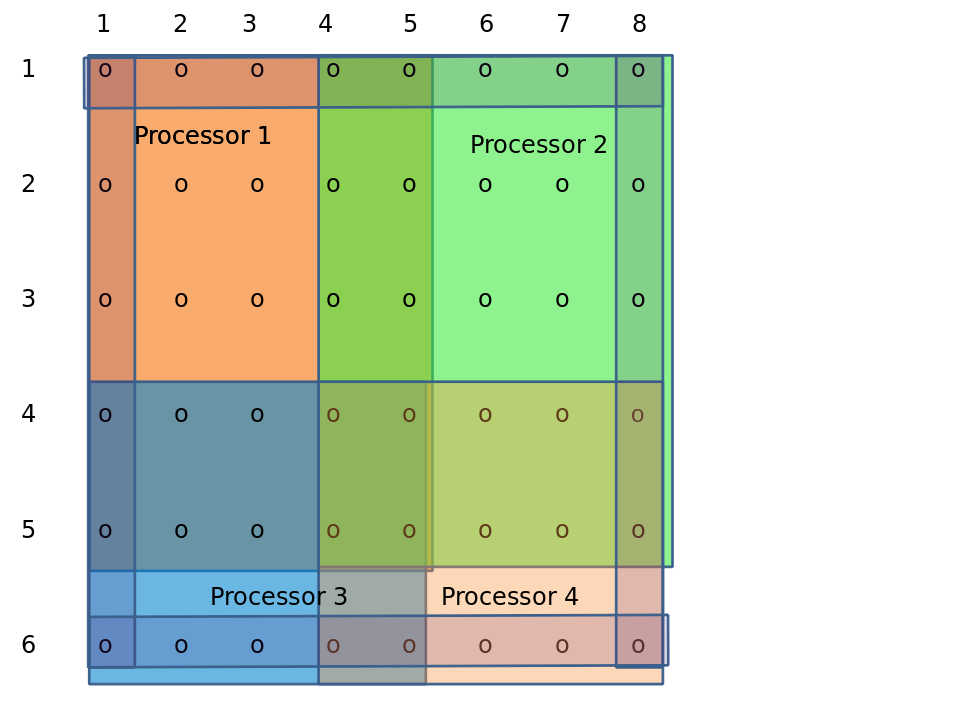
\includegraphics[width=10cm]{configuration.png}
 \caption{Configuration of Processors}
 \label{fig:configuration}
 \end{center}
 \end{figure}
 Figure  \ref{fig:configuration} is an example.In figure \ref{fig:configuration}, "o" is an element in the Psi or Omega matrix.Row 1,6 and column 1,8 are the boundaries.  Here, we have 4 processors.Processor 1 stores the part covered by red square which ranges from row 1 to 5 and column 1 to 5. Processor 2 stores the part covered by green square,which ranges from row 1 to 5 and from column 4 to 8 . Processor 3 stores the elements covered by the blue square.  But processor 1 only calculate elements from row 2 to row 4 and from column 2 to column 4.The rest elements are considered as the boundary of processor 1. Although column 5 is the boundary of processor 1,  it is not the boundary of processor 2. So processor 2 will calculate column 5 and send the value of these elements to processor 1. In the same way, processor 3 will calculate row 5 and send them to processor 1.So processor 1 will have updated value for all the elements . For the same reason, all the processors will get the new values for the matrices after one iteration.
 The criterion to stop the iteration is the maximum difference between the old matrix and the new matrix is smaller than a specific value PsiTol. So when finishing an iteration, the maximum difference between the old Psi matrix and the new Psi matrix is calculated in all the processor. We use mpi\_all\_reduce to gather the maximum value in different processors and compare them with PsiTol to determine whether to continue next iteration or not.
 

\end{document}


